\documentclass{article}\usepackage[]{graphicx}\usepackage[]{color}
%% maxwidth is the original width if it is less than linewidth
%% otherwise use linewidth (to make sure the graphics do not exceed the margin)
\makeatletter
\def\maxwidth{ %
  \ifdim\Gin@nat@width>\linewidth
    \linewidth
  \else
    \Gin@nat@width
  \fi
}
\makeatother

\definecolor{fgcolor}{rgb}{0.345, 0.345, 0.345}
\newcommand{\hlnum}[1]{\textcolor[rgb]{0.686,0.059,0.569}{#1}}%
\newcommand{\hlstr}[1]{\textcolor[rgb]{0.192,0.494,0.8}{#1}}%
\newcommand{\hlcom}[1]{\textcolor[rgb]{0.678,0.584,0.686}{\textit{#1}}}%
\newcommand{\hlopt}[1]{\textcolor[rgb]{0,0,0}{#1}}%
\newcommand{\hlstd}[1]{\textcolor[rgb]{0.345,0.345,0.345}{#1}}%
\newcommand{\hlkwa}[1]{\textcolor[rgb]{0.161,0.373,0.58}{\textbf{#1}}}%
\newcommand{\hlkwb}[1]{\textcolor[rgb]{0.69,0.353,0.396}{#1}}%
\newcommand{\hlkwc}[1]{\textcolor[rgb]{0.333,0.667,0.333}{#1}}%
\newcommand{\hlkwd}[1]{\textcolor[rgb]{0.737,0.353,0.396}{\textbf{#1}}}%
\let\hlipl\hlkwb

\usepackage{framed}
\makeatletter
\newenvironment{kframe}{%
 \def\at@end@of@kframe{}%
 \ifinner\ifhmode%
  \def\at@end@of@kframe{\end{minipage}}%
  \begin{minipage}{\columnwidth}%
 \fi\fi%
 \def\FrameCommand##1{\hskip\@totalleftmargin \hskip-\fboxsep
 \colorbox{shadecolor}{##1}\hskip-\fboxsep
     % There is no \\@totalrightmargin, so:
     \hskip-\linewidth \hskip-\@totalleftmargin \hskip\columnwidth}%
 \MakeFramed {\advance\hsize-\width
   \@totalleftmargin\z@ \linewidth\hsize
   \@setminipage}}%
 {\par\unskip\endMakeFramed%
 \at@end@of@kframe}
\makeatother

\definecolor{shadecolor}{rgb}{.97, .97, .97}
\definecolor{messagecolor}{rgb}{0, 0, 0}
\definecolor{warningcolor}{rgb}{1, 0, 1}
\definecolor{errorcolor}{rgb}{1, 0, 0}
\newenvironment{knitrout}{}{} % an empty environment to be redefined in TeX

\usepackage{alltt}
\usepackage[margin=0.5in]{geometry}
\IfFileExists{upquote.sty}{\usepackage{upquote}}{}
\begin{document}





\section*{Simulations, independence}

Consider 1,000 tests in each simulation, 200 simulations per scenario, nominal FDR = 5\%.
\\
The following 4 functions are considered for $\pi_0(x)$:
\begin{knitrout}
\definecolor{shadecolor}{rgb}{0.969, 0.969, 0.969}\color{fgcolor}

{\centering 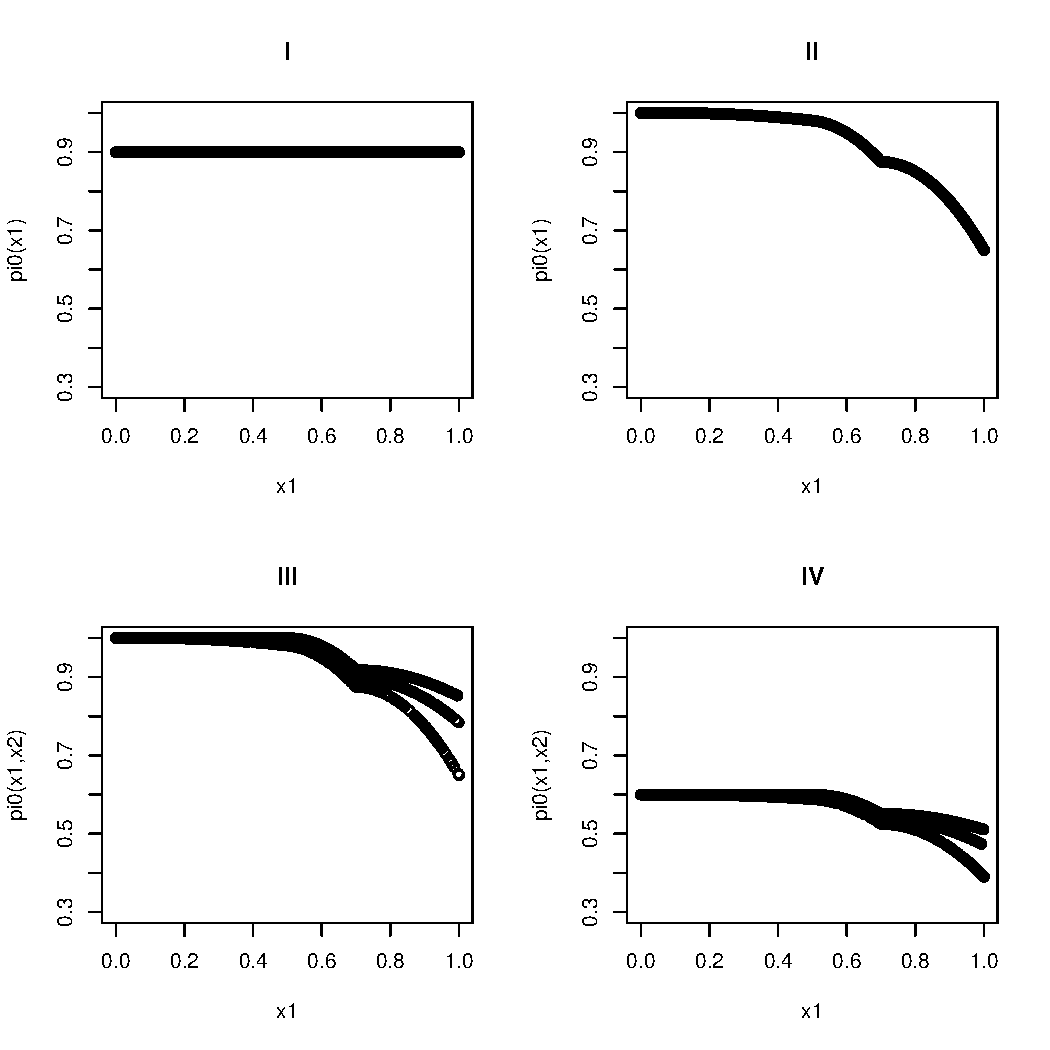
\includegraphics[width=\maxwidth]{Figures/unnamed-chunk-3-1} 

}



\end{knitrout}

\clearpage




  
  Estimated false discovery rates (FDR) and true positive rates (TPR) percentages. BL = Boca-Leek. W.S. = well-separated null and alternative, P.S. = poorly separated null and alternative. For III and IV, a dummy variable was used for $x_{2}$, along with linear or spline terms for $x_1$. Used reviewer's definition of ``well-separated" and ``poorly-separated." Used both the theoretical and empirical nulls for the Scott method. For the t-test, considered 2 groups of 6 (so 2x6 = 10 df) and used the t-statistics instead of the z-statistics for the Scott method. Extended ``well-separated" and ``poorly-separated" definition to chisquared test, generating means fom the absolute value of a normal distribution with mean 9, respectively 1. For the chisquared test, 1 df corresponds to a 2x2 table, 4 df to a 3x3 table. Used the z-values obtained from back-transforming the p-values for the Scott method in this case.
% latex table generated in R 3.3.1 by xtable 1.8-2 package
% Thu Jun 22 11:08:09 2017
\begin{table}[ht]
\centering
\begin{tabular}{lll|lllll|lllll}
  \hline
  &&& \multicolumn{5}{c}{FDR} & \multicolumn{5}{c}{TPR}\\
 $\pi_0(x)$ &  Dist. under $H_1$ & Reg. model & BL & Scott T & Scott E & Storey & BH & BL & Scott T & Scott E & Storey & BH    \\
 \hline
I & Beta(1,20) & Linear & 5.0 & 90.0 & 84.0 & 5.2 & 3.9 & 0.2 & 100.0 & 95.9 & 0.2 & 0.1 \\ 
  II & Beta(1,20) & Linear & 4.8 & 92.6 & 85.9 & 4.8 & 4.1 & 0.2 & 100.0 & 98.0 & 0.1 & 0.1 \\ 
  II & Beta(1,20) & Spline & 6.5 & 92.6 & 86.6 & 4.8 & 4.1 & 0.2 & 100.0 & 98.3 & 0.1 & 0.1 \\ 
  III & Beta(1,20) & Linear & 5.2 & 94.9 & 88.9 & 5.4 & 5.4 & 0.2 & 100.0 & 97.5 & 0.2 & 0.2 \\ 
  III & Beta(1,20) & Spline & 6.2 & 94.9 & 89.4 & 5.4 & 5.4 & 0.3 & 100.0 & 97.6 & 0.2 & 0.2 \\ 
  IV & Beta(1,20) & Linear & 6.4 & 56.7 &  & 5.1 & 3.4 & 12.2 & 100.0 &  & 5.4 & 0.3 \\ 
  IV & Beta(1,20) & Spline & 7.9 & 56.7 &  & 5.1 & 3.4 & 15.4 & 100.0 &  & 5.4 & 0.3 \\ 
   \hline
I & Norm (W.S.) & Linear & 5.0 & 5.2 & 6.6 & 4.9 & 4.4 & 51.0 & 50.9 & 49.7 & 50.8 & 49.7 \\ 
  II & Norm (W.S.) & Linear & 5.4 & 5.7 & 8.1 & 5.3 & 4.9 & 48.5 & 63.5 & 61.3 & 47.6 & 47.0 \\ 
  II & Norm (W.S.) & Spline & 5.6 & 5.9 & 8.3 & 5.3 & 4.9 & 49.3 & 63.5 & 61.5 & 47.6 & 47.0 \\ 
  III & Norm (W.S.) & Linear & 5.8 & 5.9 & 9.9 & 5.4 & 5.1 & 45.1 & 60.3 & 57.9 & 44.0 & 43.4 \\ 
  III & Norm (W.S.) & Spline & 5.9 & 6.0 & 10.1 & 5.4 & 5.1 & 45.6 & 60.9 & 58.2 & 44.0 & 43.4 \\ 
  IV & Norm (W.S.) & Linear & 5.0 & 4.9 & 2.4 & 4.7 & 2.8 & 71.6 & 71.8 & 60.6 & 71.2 & 65.4 \\ 
  IV & Norm (W.S.) & Spline & 5.2 & 5.0 & 2.4 & 4.7 & 2.8 & 72.0 & 71.9 & 60.7 & 71.2 & 65.4 \\ 
   \hline
I & T (W.S.) & Linear & 5.7 & 21.3 & 23.4 & 5.5 & 4.8 & 15.7 & 55.4 & 56.9 & 15.2 & 13.6 \\ 
  II & T (W.S.) & Linear & 4.8 & 20.7 & 23.8 & 5.0 & 4.4 & 13.0 & 64.5 & 65.5 & 11.6 & 10.6 \\ 
  II & T (W.S.) & Spline & 4.7 & 21.1 & 24.5 & 5.0 & 4.4 & 13.8 & 64.8 & 65.6 & 11.6 & 10.6 \\ 
  III & T (W.S.) & Linear & 6.2 & 26.8 & 31.0 & 5.9 & 5.4 & 9.4 & 54.6 & 54.7 & 8.2 & 7.6 \\ 
  III & T (W.S.) & Spline & 6.8 & 27.3 & 31.3 & 5.9 & 5.4 & 10.0 & 55.2 & 55.3 & 8.2 & 7.6 \\ 
  IV & T (W.S.) & Linear & 5.0 & 9.3 & 2.8 & 4.7 & 2.9 & 52.5 & 72.9 & 44.4 & 52.0 & 40.3 \\ 
  IV & T (W.S.) & Spline & 5.4 & 9.3 & 2.8 & 4.7 & 2.9 & 53.0 & 73.0 & 44.6 & 52.0 & 40.3 \\ 
   \hline
I & Chisq 1 df (W.S.) & Linear & 5.0 & 90.0 & 85.5 & 4.8 & 4.4 & 51.2 & 100.0 & 98.7 & 50.9 & 49.7 \\ 
  II & Chisq 1 df (W.S.) & Linear & 4.8 & 92.6 & 89.4 & 4.8 & 4.4 & 48.3 & 100.0 & 99.6 & 47.1 & 46.3 \\ 
  II & Chisq 1 df (W.S.) & Spline & 5.0 & 92.6 & 90.0 & 4.8 & 4.4 & 48.9 & 100.0 & 99.6 & 47.1 & 46.3 \\ 
  III & Chisq 1 df (W.S.) & Linear & 5.0 & 94.9 & 93.8 & 4.9 & 4.8 & 44.3 & 100.0 & 99.7 & 43.1 & 42.5 \\ 
  III & Chisq 1 df (W.S.) & Spline & 5.3 & 94.9 & 93.9 & 4.9 & 4.8 & 44.8 & 100.0 & 99.7 & 43.1 & 42.5 \\ 
  IV & Chisq 1 df (W.S.) & Linear & 5.1 & 56.7 &  & 4.7 & 2.8 & 71.6 & 100.0 &  & 71.1 & 65.1 \\ 
  IV & Chisq 1 df (W.S.) & Spline & 5.3 & 56.7 &  & 4.7 & 2.8 & 71.9 & 100.0 &  & 71.1 & 65.1 \\ 
   \hline
I & Chisq 4 df (W.S.) & Linear & 5.3 & 90.0 & 83.5 & 5.4 & 4.8 & 30.8 & 100.0 & 95.3 & 30.6 & 29.6 \\ 
  II & Chisq 4 df (W.S.) & Linear & 5.3 & 92.6 & 89.6 & 5.3 & 5.0 & 28.4 & 100.0 & 98.5 & 27.5 & 26.7 \\ 
  II & Chisq 4 df (W.S.) & Spline & 5.4 & 92.6 & 89.9 & 5.3 & 5.0 & 29.2 & 100.0 & 98.6 & 27.5 & 26.7 \\ 
  III & Chisq 4 df (W.S.) & Linear & 5.9 & 94.9 & 92.4 & 5.4 & 5.3 & 24.8 & 100.0 & 98.3 & 24.0 & 23.4 \\ 
  III & Chisq 4 df (W.S.) & Spline & 5.9 & 94.9 & 93.0 & 5.4 & 5.3 & 25.2 & 100.0 & 98.7 & 24.0 & 23.4 \\ 
  IV & Chisq 4 df (W.S.) & Linear & 5.1 & 56.7 & 55.9 & 4.7 & 2.8 & 52.3 & 100.0 & 98.8 & 51.7 & 44.5 \\ 
  IV & Chisq 4 df (W.S.) & Spline & 5.5 & 56.7 & 55.9 & 4.7 & 2.8 & 52.7 & 100.0 & 98.8 & 51.7 & 44.5 \\ 
   \hline
\end{tabular}
\end{table}



\end{document}
